\documentclass{amsart}
% Adapted from the supplied FirstVersion.tex (Ryuya Hora template).
% The environment-specific dmjhira font declaration is omitted for portability.
\usepackage[left=2cm,right=2cm,top=2.2cm,bottom=2.2cm]{geometry}
\usepackage[utf8]{inputenc}
\usepackage[T1]{fontenc}
\usepackage{amsfonts,amsthm,amssymb,mathtools,etoolbox,stmaryrd}
\usepackage[colorlinks=true,urlcolor=blue,linkcolor=blue,citecolor=blue]{hyperref}
\usepackage{tikz,tikz-cd}
\usetikzlibrary{calc,arrows.meta,positioning,fit,backgrounds}
\usepackage{cleveref}
\usepackage{xcolor}
\usepackage{array,booktabs,longtable,tabularx}
\usepackage{enumitem}
\usepackage{microtype}
\usepackage{xurl}
\usepackage{listings}
\usepackage[style=alphabetic,sorting=nyt,maxnames=5]{biblatex}
\renewbibmacro{in:}{}
\addbibresource{CommonBiblio20240922.bib}
\addbibresource{gsh_additions.bib}

\tikzset{pullback/.style={minimum size=1.2ex,path picture={
\draw[opacity=1,black,-,#1] (-0.5ex,-0.5ex) -- (0.5ex,-0.5ex) -- (0.5ex,0.5ex);%
}}}

\theoremstyle{plain}
\newtheorem{theorem}{Theorem}[subsection]
\newtheorem{proposition}[theorem]{Proposition}
\newtheorem{lemma}[theorem]{Lemma}
\newtheorem{corollary}[theorem]{Corollary}
\newtheorem{todo}[theorem]{Todo}
\newtheorem{conjecture}[theorem]{Conjecture}
\newtheorem{fact}[theorem]{Fact}
\newtheorem{claim}{Claim}[theorem]
\crefname{claim}{Claim}{Claims}
\renewcommand{\theclaim}{\thetheorem.\alph{claim}}

\theoremstyle{definition}
\newtheorem{example}[theorem]{Example}
\newtheorem{definition}[theorem]{Definition}
\newtheorem{notation}[theorem]{Notation}
\newtheorem{puzzle}[theorem]{Puzzle}
\newtheorem{idea}[theorem]{Idea}
\newtheorem{question}[theorem]{Question}
\newtheorem{exercise}[theorem]{Exercise}
\newtheorem{protocol}[theorem]{Protocol}

\theoremstyle{remark}
\newtheorem{remark}[theorem]{Remark}
\newtheorem{warning}[theorem]{Warning}

\newcommand{\dq}[1]{``#1''}
\newcommand{\memo}[1]{\textcolor{red}{memo: #1}}
\newcommand{\invmemo}[1]{}
\newcommand{\horamemo}[1]{\textcolor{green!60!black}{hora: #1}}
\newcommand{\para}[1]{\paragraph{\textbf{#1}}}
\newcommand{\N}{\mathbb{N}}
\newcommand{\Z}{\mathbb{Z}}
\newcommand{\Q}{\mathbb{Q}}
\newcommand{\R}{\mathbb{R}}
\newcommand{\C}{\mathcal{C}}
\newcommand{\D}{\mathcal{D}}
\newcommand{\E}{\mathcal{E}}
\newcommand{\F}{\mathbf{F}}
\renewcommand{\L}{\mathcal{L}}
\newcommand{\id}{\mathrm{id}}
\newcommand{\op}{\mathrm{op}}
\newcommand{\ob}{\mathrm{ob}}
\newcommand{\Set}{\mathbf{Set}}
\newcommand{\FinSet}{\mathbf{FinSet}}
\newcommand{\Func}[2]{[#1,#2]}
\newcommand{\abs}[1]{\left|#1\right|}
\newcommand{\demph}[1]{\textit{#1}}
\newcommand{\Pow}{\mathcal{P}}
\newcommand{\Words}[1]{#1^{\ast}}
\newcommand{\eps}{\varepsilon}
\newcommand{\sh}{\operatorname{sh}}
\newcommand{\Syn}{\operatorname{Syn}}
\newcommand{\Aper}{\mathbf{A}}
\newcommand{\Afour}{A_{4}}
\newcommand{\Afive}{A_{5}}
\newcommand{\Dicthree}{\operatorname{Dic}_{3}}
\newcommand{\heightone}{\mathsf{H}_{1}}
\newcommand{\code}[1]{\texttt{\detokenize{#1}}}
\newcommand{\status}[1]{\textsf{#1}}

\definecolor{codegray}{gray}{0.97}
\lstdefinestyle{workshop}{
  basicstyle=\ttfamily\small,
  backgroundcolor=\color{codegray},
  frame=single,
  framerule=0.2pt,
  columns=fullflexible,
  keepspaces=true,
  breaklines=true,
  showstringspaces=false,
  upquote=true,
  literate={α}{{$\alpha$}}1
}
\lstset{style=workshop}

\setlist[itemize]{topsep=3pt,itemsep=2pt,parsep=0pt}
\setlist[enumerate]{topsep=3pt,itemsep=2pt,parsep=0pt}
\setcounter{tocdepth}{2}
\setcounter{secnumdepth}{3}


\title{A Blueprint for Lean Formalization of the Generalized Star-Height Program}
\author{Ryuya Hora and the ZMC Generalized Star-Height Working Group}
\address{Prepared for group work at the ZMC conference, ZEN University}
\email{}
\date{22 July 2026}
\subjclass[2020]{68V15, 03B35, 20B35, 20J06}
\keywords{generalized star height, regular languages, syntactic monoids, finite groups, Lean, certificates, $A_5$}

\begin{document}
\begin{abstract}
This document specifies a staged Lean formalization for research on the generalized star-height problem.  It separates established results, formalization interfaces, computational certificates, and speculative research routes.  The first formal milestones are words and languages, generalized regular-expression semantics, deterministic automata, monoid recognition, syntactic congruence, and a trusted certificate boundary.  The mathematical program proceeds from published height-one constructions through the first unresolved order-twelve cases $A_4$ and $\operatorname{Dic}_3$, then to the non-solvable test case $A_5$.  Group or monoid cohomology is included only as an exploratory layer requiring a concrete map from recognition data to cochains.  The blueprint also gives theorem signatures, dependency graphs, test obligations, failure modes, and release gates for an AI-assisted workshop.
\end{abstract}
\maketitle
\tableofcontents

\section{Purpose, scope, and status discipline}

\subsection{What this blueprint is}

The goal is not to make a large formal-language library before knowing which theorem will matter.  The goal is to build the smallest reliable formal kernel that can support three kinds of research artifact:
\begin{enumerate}
  \item a checked upper-bound certificate, usually an explicit generalized regular expression of star-height at most one;
  \item a formalized transport theorem, such as closure under an inverse morphism or a substitution;
  \item a sound lower-bound invariant or game, should one be found.
\end{enumerate}
The formalization is therefore organized around theorem interfaces and verification boundaries rather than around encyclopedic coverage.

\subsection{Status labels}

Every substantial claim in the repository is assigned one of the following labels.
\begin{center}
\begin{tabularx}{0.94\textwidth}{@{}lX@{}}
\toprule
\status{PROVED} & proved in Lean or in a complete argument stored in the repository, with a location;\\
\status{CITED} & taken from a primary source whose exact hypotheses have been checked;\\
\status{COMPUTED} & obtained by a deterministic program with a run manifest and independently checkable output;\\
\status{CONJECTURAL} & a precise mathematical statement not proved;\\
\status{SPECULATIVE} & a research vocabulary or route that is not yet a precise conjecture;\\
\status{REFUTED} & false, with an explicit counterexample or source correction;\\
\status{UNREVIEWED} & generated or imported and awaiting audit.\\
\bottomrule
\end{tabularx}
\end{center}
A Lean declaration containing \code{sorry} is an interface and remains \status{UNREVIEWED}.  A finite search that fails to find an expression remains \status{COMPUTED}; it is not a lower bound.

\subsection{Current mathematical status}

A generalized regular expression permits complement in addition to the ordinary regular operations.  The decision problem asks for the minimum nesting depth of Kleene star.  No regular language of generalized star-height greater than one is known in the surveyed literature; the decision problem remains open \cite{pinStraubingTherien1992,bourne2017counting,placeZeitoun2017generic}.  This is distinct from restricted star height, where complement is unavailable and the decision problem was settled by Hashiguchi \cite{hashiguchi1988algorithms}.

The workshop adopts the following north-star conjecture.
\begin{conjecture}[Height-one collapse]\label{conj:collapse}
For every finite alphabet $A$ and every regular language $L\subseteq A^\ast$, the generalized star-height of $L$ is at most one.
\end{conjecture}
A proof of \cref{conj:collapse} would reduce exact height computation to the established height-zero question: a regular language is star-free exactly when its syntactic monoid is aperiodic \cite{schutzenberger1965finite,mcnaughtonPapert1971counterfree}.  A counterexample would need an explicit regular language and a rigorous argument excluding every height-one expression.

\section{Mathematical objects to formalize}

\subsection{Words and languages}

Fix a type $A$ of letters.  A word is a finite list, so the free monoid is
\[
  A^\ast := \operatorname{List}(A), \qquad 1_{A^\ast}=\eps,
\]
with multiplication given by concatenation.  A language is a subset $L\subseteq A^\ast$.  The formalization uses
\begin{lstlisting}[language={},caption={Core Lean representations.}]
abbrev Word (A : Type u) := List A
abbrev Language (A : Type u) := Set (Word A)
\end{lstlisting}
This choice makes the empty word and complement universe explicit.  In particular, $L^c$ always means $A^\ast\setminus L$, never complement inside a finite sample of words.

Language concatenation and star are semantic definitions:
\[
LK=\{uv\mid u\in L,\ v\in K\},\qquad
L^\ast=\bigcup_{n\geq 0}L^n,\quad L^0=\{\eps\}.
\]
The first tests must include the empty alphabet, $\varnothing^\ast=\{\eps\}$, and associativity of concatenation.

\subsection{Generalized regular expressions}

\begin{definition}
For a finite alphabet $A$, the type $\operatorname{GRegex}(A)$ is inductively generated by
\[
0,\quad \eps,\quad a\ (a\in A),\quad r+s,\quad rs,\quad r^c,\quad r^\ast.
\]
Its denotation $\llbracket r\rrbracket\subseteq A^\ast$ is defined compositionally.
\end{definition}

The syntax-tree height is
\[
\begin{aligned}
\sh(0)=\sh(\eps)=\sh(a)&=0,\\
\sh(r+s)=\sh(rs)&=\max(\sh(r),\sh(s)),\\
\sh(r^c)&=\sh(r),\\
\sh(r^\ast)&=1+\sh(r).
\end{aligned}
\]
This is not yet the height of a language.

\begin{definition}[Semantic upper bound]\label{def:hasheight}
For $L\subseteq A^\ast$ and $n\in\N$, write
\[
  \operatorname{HasHeightAtMost}(L,n)
  :\Longleftrightarrow
  \exists r,\ \llbracket r\rrbracket=L\text{ and }\sh(r)\leq n.
\]
\end{definition}
This existential formulation avoids defining a minimum over an inhabited set before regularity has been established.  A later theorem may prove existence and uniqueness of the least $n$ for regular $L$.

\subsection{Automata}

A deterministic automaton consists of a state type $Q$, transition $\delta:Q\times A\to Q$, start state $q_0$, and accepting set $F\subseteq Q$.  The recursive run function must satisfy
\[
  \delta^\ast(q,uv)=\delta^\ast(\delta^\ast(q,u),v).
\]
This lemma is the first nontrivial compile target because it occurs in every proof relating automata, recognition, and contexts.  Finiteness should be a separate hypothesis: the core semantics does not need $Q$ finite, while equivalence algorithms do.

\subsection{Monoid recognition}

A finite monoid $M$ recognizes $L\subseteq A^\ast$ when there is a monoid morphism
\[
  \varphi:A^\ast\longrightarrow M
\]
and a subset $P\subseteq M$ with $L=\varphi^{-1}(P)$.  Surjectivity is not part of recognition.  If desired, one may replace $M$ by the image afterward.

\begin{warning}
\dq{$L$ is recognized by $M$} does not mean that the syntactic monoid of $L$ is isomorphic to $M$.  Recognition is existential and is stable under passage to suitable divisors; the syntactic monoid is the minimal recognizing quotient.
\end{warning}

The central group-language property is formalized as
\[
\heightone(G):\Longleftrightarrow
\text{every language recognized by the finite group $G$ has height at most one}.
\]
All alphabet, finiteness, morphism, and accepting-set quantifiers must be visible in the Lean definition.

\subsection{Syntactic congruence}

For a language $L\subseteq A^\ast$, define
\[
  u\equiv_L v
  \quad\Longleftrightarrow\quad
  \forall x,y\in A^\ast,\ xuy\in L\Longleftrightarrow xvy\in L.
\]
The proof order is important:
\begin{enumerate}
  \item prove reflexivity, symmetry, and transitivity;
  \item prove compatibility with adding the same prefix and suffix;
  \item prove two-sided compatibility with concatenation;
  \item only then construct the quotient monoid $A^\ast/\!\equiv_L$.
\end{enumerate}
Delaying the quotient isolates elementary list algebra from API-sensitive quotient machinery.

\section{Source-audited mathematical baseline}

\subsection{Height zero}

Sch\"utzenberger's theorem gives the algebraic base case: a regular language is star-free if and only if its syntactic monoid is aperiodic \cite{schutzenberger1965finite}.  McNaughton and Papert supply the counter-free automata and first-order logical perspective \cite{mcnaughtonPapert1971counterfree}.  The initial Lean artifact is a theorem interface, not an attempt to formalize all equivalences at once.

\subsection{Pin--Straubing--Th\'erien}

The principal algebraic source is \cite{pinStraubingTherien1992}.  Its relevant contributions include bounded-height closure under specified quotients, inverse alphabetic morphisms, and injective star-free substitutions; height-one results for languages recognized by commutative groups; extensions to nilpotent groups of class at most two; and a family involving semidirect products by elementary abelian $2$-groups.  Exact formal statements must be extracted from the paper before use: an abstract or survey paraphrase is not enough for a Lean theorem.

The proof architecture can be separated into three layers:
\[
\boxed{\text{explicit counts}}
\longrightarrow
\boxed{\text{group/monoid decomposition}}
\longrightarrow
\boxed{\text{closure transport}}.
\]
This separation is ideal for formalization because each layer has independent tests.

\subsection{Factor-count certificates}

Bourne and Ru\v{s}kuc give explicit exact-count and modular-count constructions and apply them to Rees zero-matrix semigroups over abelian groups \cite{bourneRuskuc2016}.  These expressions are preferable early formalization targets to a purely existential theorem: a concrete expression can be checked by automata equivalence and later imported as a Lean certificate.

\subsection{The order-twelve barrier}

Bourne's thesis records that, in the finite-group ladder under consideration, all groups of order below $12$ are covered by preceding results; the remaining order-twelve cases are
\[
  A_4\cong (C_2\times C_2)\rtimes C_3,
  \qquad
  \operatorname{Dic}_3\cong C_3\rtimes C_4
\]
in the thesis notation \cite{bourne2017counting}.  The attempted extension of an $A\rtimes C_2$ argument to $A\rtimes C_3$ fails because the required decomposition of words into consecutive non-overlapping factors is not unique.

This changes the milestone order.  $A_5$ is a strategically important simple non-solvable group, but it is not the first unresolved group-order case.  A theorem for $A_4$, $\operatorname{Dic}_3$, or a precisely specified $A\rtimes C_3$ family is the lower-risk research target.

\section{Repository architecture}

\subsection{Dependency graph}

\begin{center}
\resizebox{0.98\textwidth}{!}{%
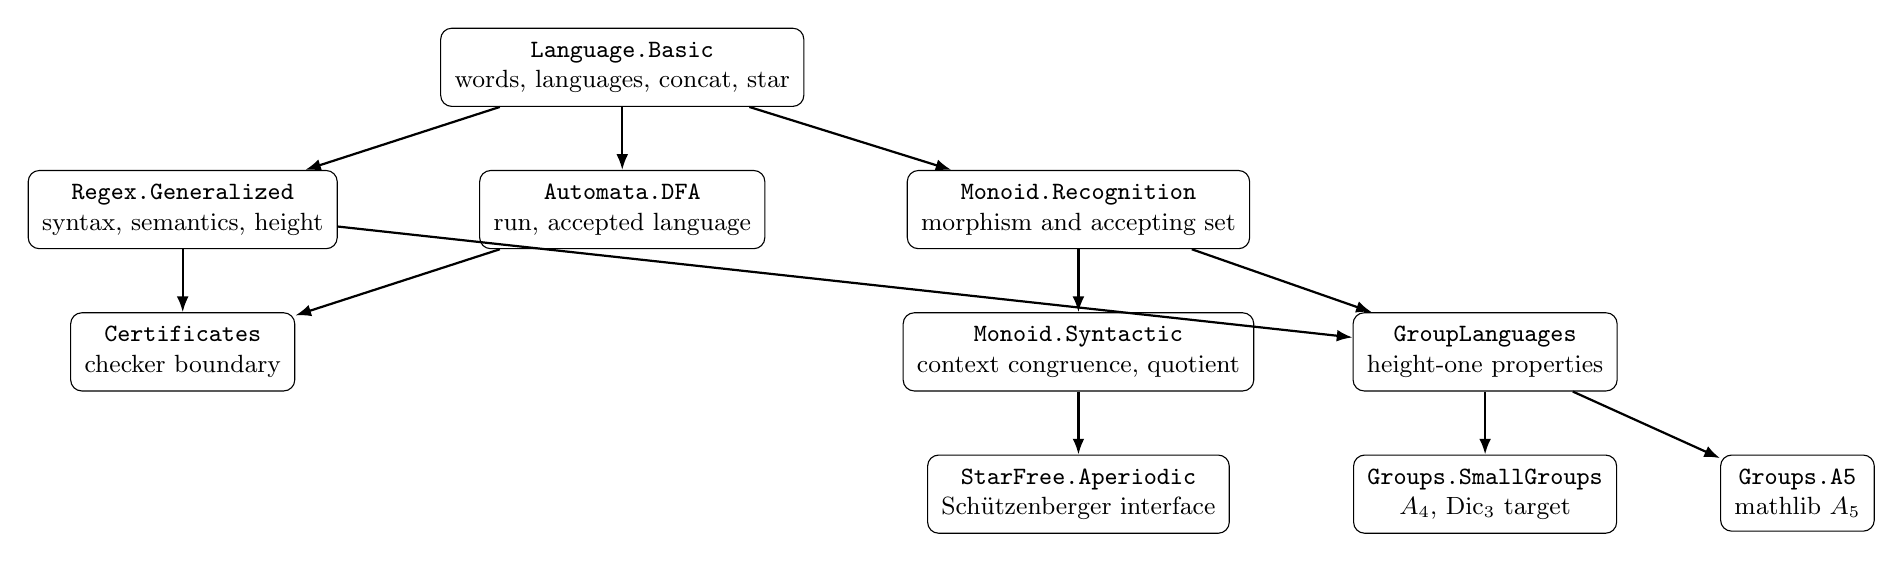
\begin{tikzpicture}[
  node distance=8mm and 13mm,
  box/.style={draw,rounded corners,align=center,inner sep=5pt,font=\small},
  arr/.style={-{Latex[length=2mm]},thick}
]
\node[box] (lang) {\code{Language.Basic}\\words, languages, concat, star};
\node[box,below left=of lang] (regex) {\code{Regex.Generalized}\\syntax, semantics, height};
\node[box,below=of lang] (dfa) {\code{Automata.DFA}\\run, accepted language};
\node[box,below right=of lang] (rec) {\code{Monoid.Recognition}\\morphism and accepting set};
\node[box,below=of regex] (cert) {\code{Certificates}\\checker boundary};
\node[box,below=of rec] (syn) {\code{Monoid.Syntactic}\\context congruence, quotient};
\node[box,below=of syn] (sf) {\code{StarFree.Aperiodic}\\Sch\"utzenberger interface};
\node[box,below right=of rec] (groups) {\code{GroupLanguages}\\height-one properties};
\node[box,below=of groups] (small) {\code{Groups.SmallGroups}\\$A_4$, $\operatorname{Dic}_3$ target};
\node[box,below right=of groups] (a5) {\code{Groups.A5}\\mathlib $A_5$};
\draw[arr] (lang)--(regex);
\draw[arr] (lang)--(dfa);
\draw[arr] (lang)--(rec);
\draw[arr] (regex)--(cert);
\draw[arr] (dfa)--(cert);
\draw[arr] (rec)--(syn);
\draw[arr] (syn)--(sf);
\draw[arr] (regex)--(groups);
\draw[arr] (rec)--(groups);
\draw[arr] (groups)--(small);
\draw[arr] (groups)--(a5);
\end{tikzpicture}%
}
\end{center}

The graph is intentionally shallow.  Cohomology is absent because no concrete theorem yet requires it.

\subsection{Module contracts}

\begin{longtable}{@{}p{0.25\textwidth}p{0.67\textwidth}@{}}
\toprule
Module & Contract\\
\midrule
\endhead
\code{Language.Basic} & Define words and languages, semantic operations, and elementary membership lemmas.  No automata or finiteness assumptions.\\
\code{Regex.Generalized} & Define the generalized syntax, denotation, syntactic star height, regularity, star-free, and semantic height upper bounds.\\
\code{Automata.DFA} & Define deterministic run and accepted language; prove run over append.  Algorithms are placed in a later finite-state file.\\
\code{Monoid.Recognition} & Define recognition as inverse image under a list-monoid homomorphism.  Keep surjectivity optional.\\
\code{Monoid.Syntactic} & Prove contextual equivalence is a two-sided congruence; construct quotient monoid only after this proof.\\
\code{StarFree.Aperiodic} & Define aperiodicity and expose a precise interface for Sch\"utzenberger's theorem.\\
\code{Certificates} & Mirror a finite expression/DFA certificate and prove checker soundness.  Generated expressions remain untrusted.\\
\code{GroupLanguages.Basic} & State $\heightone(M)$ and $\heightone(G)$ with all quantifiers.\\
\code{Groups.SmallGroups} & Give a concrete $A_4$ model and a vetted canonical model or presentation for $\operatorname{Dic}_3$.\\
\code{Groups.A5} & Reuse \code{alternatingGroup (Fin 5)} and existing simplicity/subgroup infrastructure from mathlib \cite{mathlibAlternating2026}.\\
\bottomrule
\end{longtable}

\section{Certificate-first verification}

\subsection{Why certificates are necessary}

An AI or enumerator can propose a height-one expression much faster than humans can inspect a large Boolean regular expression.  The generator should therefore be outside the trusted base.  It returns a finite certificate containing the alphabet, abstract syntax tree, claimed height, and target DFA.  A small checker:
\begin{enumerate}
  \item parses the expression;
  \item computes syntax-tree height;
  \item compiles the expression to a complete DFA, including complement;
  \item minimizes or otherwise checks equivalence with the target DFA;
  \item returns a shortest distinguishing word when equivalence fails.
\end{enumerate}

\begin{center}
\resizebox{0.98\textwidth}{!}{%
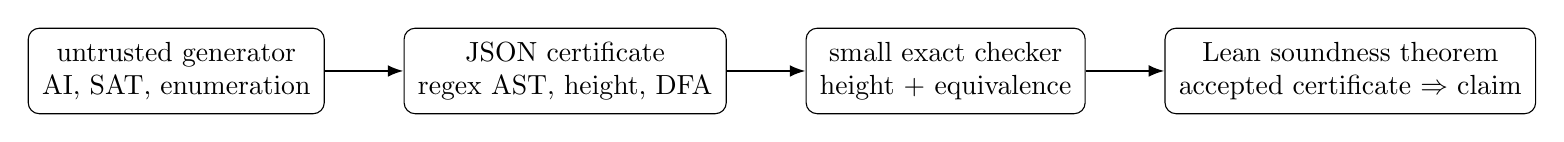
\begin{tikzpicture}[node distance=10mm,box/.style={draw,rounded corners,align=center,inner sep=5pt},arr/.style={-{Latex[length=2mm]},thick}]
\node[box] (gen) {untrusted generator\\AI, SAT, enumeration};
\node[box,right=of gen] (json) {JSON certificate\\regex AST, height, DFA};
\node[box,right=of json] (check) {small exact checker\\height + equivalence};
\node[box,right=of check] (lean) {Lean soundness theorem\\accepted certificate $\Rightarrow$ claim};
\draw[arr] (gen)--(json);
\draw[arr] (json)--(check);
\draw[arr] (check)--(lean);
\end{tikzpicture}%
}
\end{center}

The bootstrap contains a standard-library-only Python implementation of the first three stages.  It compiles generalized expressions by deterministic and $\eps$-NFA constructions rather than by bounded-word testing.  Its tests include a star-free expression for words ending in $a$ and a height-one expression for parity of the number of $a$'s.  This program is auditable but not part of Lean's trusted kernel.

\subsection{Lean soundness shape}

The eventual theorem should have the form
\begin{lstlisting}[language={},caption={Soundness boundary, schematic Lean.}]
theorem checker_sound
  (C : RegexCertificate A Q)
  (h : check C = true) :
  HasHeightAtMost C.target.language C.claimedHeight
\end{lstlisting}
The difficult theorem is not the last implication; it is proving that the Boolean checker implements denotation, height, and automata equivalence correctly.  Reflection can then verify large generated expressions without trusting the generator.

\subsection{Reproducibility metadata}

Every nontrivial computational run records:
\[
\text{commit hash},\quad
\text{prompt/input hash},\quad
\text{toolchain},\quad
\text{resource bounds},\quad
\text{output hash},\quad
\text{rerun command}.
\]
A negative bounded search may be useful as a bug detector or prioritization signal, but its claim is only that no certificate was found within the stated search space.

\section{Closure theorems as reusable formal infrastructure}

\subsection{Operations}

The Pin--Straubing--Th\'erien program transports explicit expressions through language operations.  Each formal closure theorem needs an exact syntactic constructor or a semantics-preserving transformation.  Priority operations are:
\begin{enumerate}
  \item left and right quotient by a word;
  \item inverse image under alphabetic morphisms;
  \item injective star-free substitutions under the source's exact hypotheses;
  \item Boolean operations;
  \item products or wreath-product constructions used in the algebraic decomposition.
\end{enumerate}

The formal result should construct a certificate, not merely show existence whenever the paper supplies an explicit construction.  For example:
\begin{lstlisting}[language={},caption={Preferred shape for a transport theorem.}]
def inverseAlphabeticCertificate
  (f : A -> B) (r : GRegex B) : GRegex A := ...

theorem denote_inverseAlphabeticCertificate : ...
theorem height_inverseAlphabeticCertificate :
  (inverseAlphabeticCertificate f r).starHeight <= r.starHeight := ...
\end{lstlisting}
This split makes semantics and height control independently testable.

\subsection{Do not overstate closure}

A natural-language sentence such as \'bounded height is closed under substitution\' is unsafe.  Formalization must expose whether the morphism is alphabetic, non-erasing, injective, or star-free; whether the operation is direct or inverse image; and whether the bound is preserved exactly or increased by a constant.  The source-audit task precedes the Lean task.

\section{Small finite groups before $A_5$}

\subsection{$A_4$ and $\operatorname{Dic}_3$}

The small-group track should encode recognition data for a fixed finite group independently of any global theorem.  For $A_4$, mathlib's alternating-group model is immediate.  For $\operatorname{Dic}_3$, the group lead and Lean lead must agree on a canonical model: a semidirect product $C_3\rtimes C_4$, a permutation subgroup, or a presented finite group with a proved equivalence.

The intended theorem interface is
\begin{lstlisting}[language={},caption={Group-language milestone.}]
def HeightOneForGroup (G : Type v) [Group G] : Prop :=
  forall (A : Type u) [Fintype A] [DecidableEq A],
    forall R : Recognition A G,
      HasHeightAtMost R.language 1
\end{lstlisting}
The proof should expose an algorithm or construction mapping recognition data to an expression certificate whenever possible.

\subsection{Repairing the $C_3$ obstruction}

The documented failure is not merely \'the proof is hard\': it is a specific loss of unique factorization.  Formalization can help by turning the attempted factorization into a predicate and producing minimal ambiguous words.  Replacement mechanisms should be tested separately:
\begin{itemize}
  \item a canonical parsing automaton with finite synchronization state;
  \item an unambiguous rational transduction;
  \item marked factorization forests;
  \item bounded-overlap inclusion--exclusion;
  \item a proof that no parser of a specified finite-state normal form can work.
\end{itemize}
A no-go theorem for a precise normal form is a legitimate result and prevents repeated AI rediscovery of the same failure.

\section{The $A_5$ track}

\subsection{Scope}

Mathlib provides $A_5$ as \code{alternatingGroup (Fin 5)} and proves simplicity \cite{mathlibAlternating2026}.  This removes routine group construction but not the formal-language theorem.  Proving $\heightone(A_5)$ would show that height-one methods reach a non-solvable recognizing group; it would not settle \cref{conj:collapse}.

\subsection{Concrete finite data}

The formal layer may safely compute or import checked tables for:
\begin{itemize}
  \item the five conjugacy classes: identity, double transpositions, $3$-cycles, and two classes of $5$-cycles;
  \item maximal subgroup types $A_4$, $D_5$, and $S_3$;
  \item the natural action on five points and actions on cosets of selected subgroups;
  \item restriction of a recognition morphism to preimages of subgroup/coset data.
\end{itemize}
These tables are research coordinates, not a proof.  The central missing operation is a sound gluing theorem turning local certificates into a global certificate.

\subsection{Restriction/gluing matrix}

\begin{center}
\begin{tabularx}{0.96\textwidth}{@{}lXXX@{}}
\toprule
Local object & Existing language mechanism & Algebraic data & Required global artifact\\
\midrule
cyclic $C_2,C_3,C_5$ & modular counts & characters/cyclic quotients & compatible expression certificates\\
Klein four & abelian and class-two formulas & elementary $2$-group action & overlap control inside $A_4$\\
$S_3,D_5$ & semidirect by $C_2$ families & normal cyclic subgroup & restriction/transfer formula\\
$A_4$ & unresolved $C_3$ extension case & $V_4\rtimes C_3$ & repaired parser or obstruction\\
whole $A_5$ & none known & simple group, coset actions & a gluing theorem or lower-bound invariant\\
\bottomrule
\end{tabularx}
\end{center}

\section{Cohomology: formalize only after a bridge exists}

\subsection{What cohomology could organize}

For an extension
\[
1\longrightarrow N\longrightarrow G\longrightarrow Q\longrightarrow 1,
\]
low-dimensional group cohomology records invariants, crossed homomorphisms, and extension classes; the Lyndon--Hochschild--Serre spectral sequence organizes their interaction \cite{brown1982cohomology,weibel1994homological}.  A useful language theorem might have the schematic form
\[
\heightone(N)+\heightone(Q)+\text{controlled cocycle}
\Longrightarrow \heightone(G).
\]
This formula is only a research prompt until every term after the plus signs is defined in language-theoretic data.

\subsection{Mandatory bridge data}

Before importing a cohomology library, require:
\begin{enumerate}
  \item a specific coefficient module $V$ and explicit $G$-action;
  \item a map from a word, automaton path, transition count, or accepting fiber to a cochain;
  \item a proof of the cocycle identity;
  \item a theorem describing at least one generalized-expression constructor under this map;
  \item an example where the class is nontrivial and an example where it vanishes.
\end{enumerate}
Without these, \'use the LHS spectral sequence\' is vocabulary rather than a mathematical mechanism.

\subsection{Candidate coefficient objects}

Candidates include permutation modules on cosets or states, functions on accepting fibers, the augmentation ideal of a group algebra, modules generated by transition-count functions, and bimodules attached to syntactic monoids.  Each candidate should be attacked first: complement or concatenation may destroy the proposed invariant.  A counterexample at this stage is valuable.

\section{A lower-bound formalization track}

Upper-bound constructions dominate the known finite-group program.  A disproof of height-one collapse requires a language invariant satisfied by all height-one expressions.  The formal interface should mirror an induction on syntax:
\begin{enumerate}
  \item base cases for $0,\eps$, and letters;
  \item closure under union and complement;
  \item closure or controlled composition under concatenation;
  \item one-level star applied only to star-free operands.
\end{enumerate}
The last two clauses carry the burden.  A proposed invariant should be tested against known height-one group languages before candidate search begins.

Possible---but currently speculative---forms include an expression game, profinite identities, a finite-index congruence, a topological invariant of the relevant Boolean algebra, or a cohomological obstruction with a proved constructor calculus.  Formalization is useful because it forces the claimed closure theorem to expose every assumption.

\section{Testing and review plan}

\subsection{Unit tests}

The first test suite includes:
\begin{itemize}
  \item empty and singleton alphabets;
  \item $\varnothing$, $\{\eps\}$, universal language, and singleton letters;
  \item $\varnothing^\ast=\{\eps\}$ and $\{\eps\}^\ast=\{\eps\}$;
  \item run-over-append for automata;
  \item recognition by the trivial monoid;
  \item contextual equivalence on a language with a two-state minimal automaton;
  \item a star-free certificate using complement of the empty language as $A^\ast$;
  \item a height-one parity certificate;
  \item a deliberately false DFA certificate returning a shortest witness.
\end{itemize}

\subsection{Property and finite exhaustive tests}

For small finite alphabets and state sets, executable tests may compare:
\begin{itemize}
  \item expression semantics and compiled automata up to a bounded word length, as a bug detector only;
  \item direct DFA product operations and language Boolean operations;
  \item syntactic-equivalence classes computed from a minimal DFA;
  \item group morphism evaluation and automaton transition monoids.
\end{itemize}
Bounded testing supplements, but never replaces, the exact checker or Lean proof.

\subsection{Adversarial checklist}

Every theorem-level review asks:
\begin{enumerate}
  \item Is star height generalized or restricted?
  \item Is a syntax height being mistaken for the language minimum?
  \item Is complement relative to the correct $A^\ast$?
  \item Is the empty word handled?
  \item Is recognition being confused with syntactic-monoid equality?
  \item Are inverse morphism, quotient, subgroup, and divisor directions correct?
  \item Does a factorization claim prove uniqueness or unambiguity?
  \item Is local subgroup information being glued without a theorem?
  \item Is a finite search being used as a lower bound?
  \item Does every cited theorem match the exact hypotheses?
\end{enumerate}

\section{Milestones and acceptance gates}

\subsection{Conference milestone}

A realistic two-day goal is:
\begin{quote}
Compile the core definitions; verify the Python certificate examples; reconstruct one published height-one construction; and isolate the $C_3$ factorization failure as a precise predicate with an explicit ambiguity.
\end{quote}
A new $A_4$ or $A_5$ theorem is an ambitious bonus, not a scheduling assumption.

\subsection{Twelve-week sequence}

\begin{center}
\begin{tabularx}{0.95\textwidth}{@{}lXl@{}}
\toprule
Weeks & Deliverable & Gate\\
\midrule
1--2 & compiling foundation and certificate tests & clean CI, source/semantics review\\
3--4 & one Bourne--Ru\v{s}kuc expression encoded & exact DFA equivalence certificate\\
5--6 & $A\rtimes C_2$ dependency graph and $C_3$ ambiguity suite & independent reconstruction\\
7--8 & parsing repair or no-go theorem & prover/breaker agreement\\
9--10 & $A_5$ subgroup/coset matrix and one concrete bridge candidate & no unsupported gluing claim\\
11--12 & preprint-grade lemma/theorem or obstruction report & external domain review and clean build\\
\bottomrule
\end{tabularx}
\end{center}

\subsection{Announcement gate}

A result advertised as Lean-formalized must build under the pinned toolchain with no undeclared \code{sorry} or \code{axiom}.  A mathematical resolution additionally requires a complete dependency graph, source audit, independent reconstruction, adversarial review, deterministic reproduction of computations, and external expert checking.  The layered review described in OpenAI's public unit-distance report is a useful model: automated generation and grading were followed by internal human examination, external specialists, and human-edited exposition \cite{openaiUnitDistance2026}.  The lesson is the independence of verification layers, not that an AI grade is sufficient.

\section{AI-assisted proof engineering}

\subsection{Prompt architecture}

Durable project instructions belong in small repository files such as \code{AGENTS.md}; tests and linters enforce them \cite{openaiAgentsMD2026}.  Individual tasks must freeze a claim, name nonexamples, list required artifacts, and give a verification command.  Anthropic's engineering guidance favors simple composable workflows before elaborate autonomous architectures and emphasizes executable feedback and context management \cite{anthropicEffectiveAgents2024,anthropicClaudeBestPractices2026}.

The public Jacobian prompt is useful for its process design: multiple incompatible routes, delayed convergence, theorem-strength missing lemmas, adversarial passes, and a final synthesis phase \cite{jacobianPrompt2026}.  For a resource-constrained workshop, use fewer agents but preserve mechanism-level diversity and a protected verification budget.

\subsection{Lean version policy}

The repository pins Lean and mathlib to version $4.32.0$, the stable Lean release dated 13 July 2026 in the official release notes \cite{leanReleaseNotes2026}.  The Lake file uses a fixed mathlib revision and the bootstrap invokes the documented cache command \code{lake exe cache get} \cite{mathlibDependency2026}.  Toolchain upgrades occur on a separate branch with a complete build and API-change log.

\section{Risk register}

\begin{longtable}{@{}p{0.21\textwidth}p{0.31\textwidth}p{0.38\textwidth}@{}}
\toprule
Risk & Symptom & Mitigation / acceptance test\\
\midrule
\endhead
Wrong problem & restricted-star-height theorem cited as generalized & every claim carries a height convention; source audit\\
Syntax/semantics confusion & one expression's height presented as a lower bound & use \cref{def:hasheight}; lower bounds require universal exclusion\\
Recognition confusion & theorem assumes syntactic monoid equals a chosen group & formalize recognition data and image reduction explicitly\\
Quotient fragility & time lost on quotient APIs before congruence lemmas & prove list/context compatibility first\\
Parser illusion & $C_3$ argument silently assumes unique factors & finite ambiguity suite and explicit parser theorem\\
Cohomology by analogy & spectral sequence named without a coefficient object & block imports until mandatory bridge data exists\\
Search overclaim & no small expression found & label as bounded computation with manifest\\
Formalization theater & polished PDF but Lean contains holes & proof-hole linter and clean CI gate\\
Agent convergence & all agents repeat the favored route & preserve early independence and approach registry\\
Context exhaustion & long transcript replaces durable state & checkpoints and task directories\\
Social pressure & premature announcement or invisible verification labor & independent referee, contribution log, release checklist\\
\bottomrule
\end{longtable}

\appendix
\section{Initial proof-obligation map}

\begin{longtable}{@{}p{0.17\textwidth}p{0.48\textwidth}p{0.25\textwidth}@{}}
\toprule
ID & Obligation & Acceptance\\
\midrule
\endhead
L-WORD-001 & core language operations and membership lemmas & file compiles\\
L-REGEX-001 & generalized syntax, semantics, height & file compiles; edge cases reviewed\\
L-DFA-001 & automaton run and append theorem & file compiles; smoke theorem\\
L-REC-001 & monoid recognition & source notation comparison\\
L-SYN-001 & syntactic setoid and two-sided congruence & all congruence lemmas compile\\
L-SYN-002 & quotient monoid & multiplication well-defined\\
L-SF-001 & Sch\"utzenberger interface & exact source theorem mapped\\
L-CERT-001 & verified certificate checker & acceptance implies language equality and height bound\\
L-GRP-001 & group-language height-one property & all quantifiers approved\\
L-A5-001 & $A_5$ model and library facts & pinned mathlib build\\
M-C3-FAIL-001 & explicit factorization ambiguity & word/factors independently checked\\
N-LOWER-001 & height-one invariant & closure under every constructor\\
\bottomrule
\end{longtable}

\section{Definition acceptance sheet}

Before merging a definition, the domain lead and Lean lead answer:
\begin{enumerate}
  \item What mathematical object does the type represent?
  \item Which finiteness and decidability assumptions are intrinsic, and which are algorithmic?
  \item What is the ambient complement universe?
  \item What are the empty and degenerate cases?
  \item Which equality is definitional and which requires a theorem?
  \item What is the smallest theorem that exercises the definition?
  \item Does the definition force a later theorem to use choice or quotients unnecessarily?
  \item Is there an executable representation and a semantic representation, and how are they related?
\end{enumerate}

\subsection*{Acknowledgement}

The document uses the package, theorem-environment, bibliography, and macro organization of the supplied Ryuya Hora \code{FirstVersion.tex} template, adapted only for portable fonts and workshop-specific packages.  The project should credit separately the mathematical, counterexample, formalization, source-audit, and integration contributions recorded in \code{CONTRIBUTIONS.md}.

\printbibliography
\end{document}
